\chapter{Technical Description}


Since this thesis is part of the Genetic and Evolutionary Computation Conference 2015, the conference has provided all the contestants with an API available on a GitHub. API's for different programming languages are provided, but the Java API will be used in this thesis. The API includes an implementation of a simple genetic algorithm, an evaluation method and ten different wind scenarios. This section will give an explanation of the provided API, display the results from a few test simulations (which will not be included in the final thesis), and discuss future work.


\section{API}


A class diagram of the provided API is displayed in figure \ref{Class Diagram}.


\begin{figure}
\begin{center}
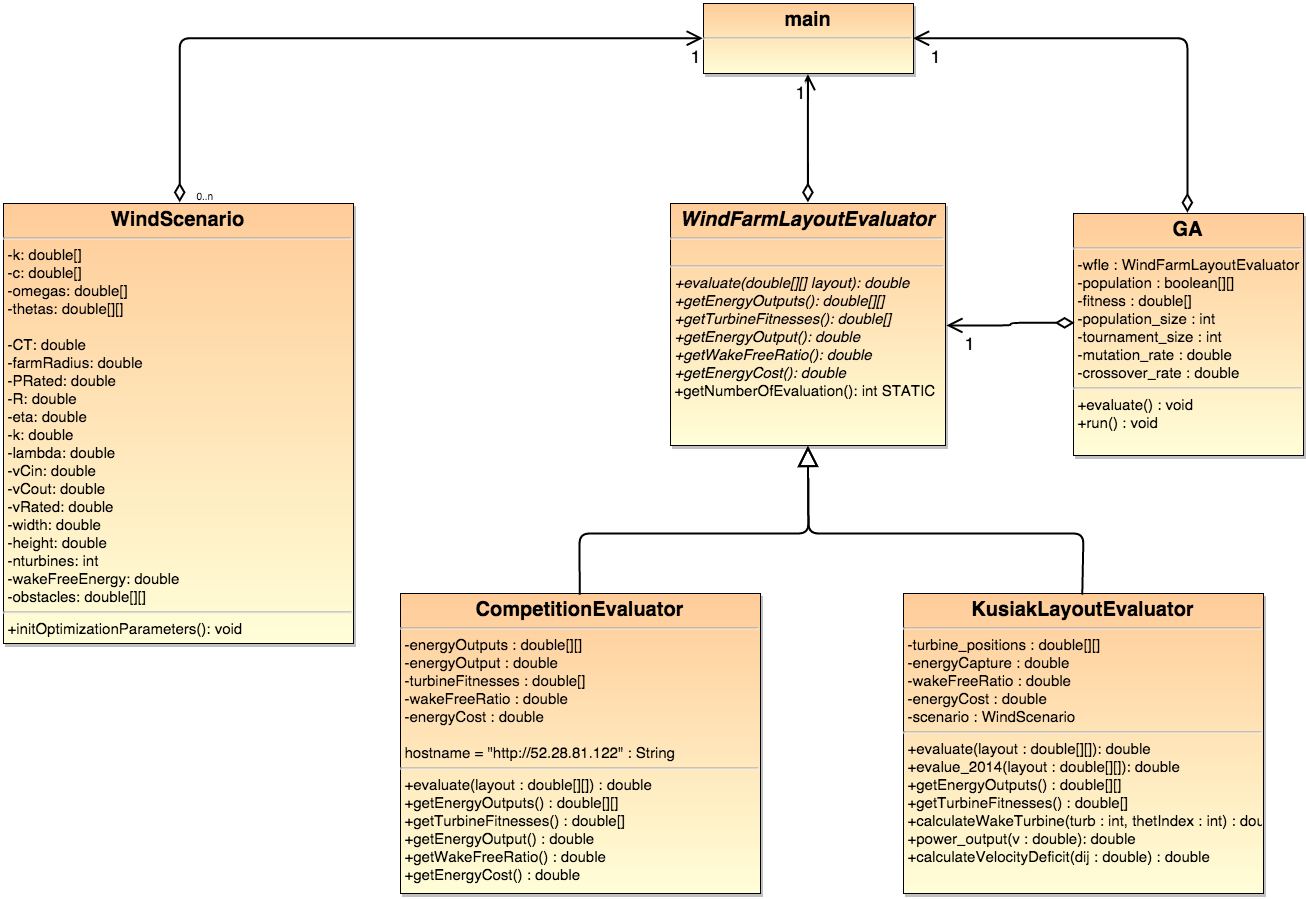
\includegraphics[scale=0.5]{images/Class Diagram}
\caption{Class diagram of the API provided på GECCO 2015.}
\label{Class Diagram}
\end{center}
\end{figure}


